% !TEX encoding = UTF-8 Unicode

%% LaTeX2e file `appendix.tex'
%% generated by the `filecontents' environment
%% from source `CLaTeX' on 2012/04/26.
%%


%\chapter{Glossary}

%\gls{naiive} \gls{computer}

\chapter{Symbols}

\begin{table}[htdp]
\begin{center}
\begin{tabular}{lccccc}
Name	& Atom 	& Negation		& Conjunction		& Disjunction		&  Implication \\
		&  		& NOT		& AND		& OR		&   \\
ASCII 	& p,q,r 	& ! 			& \& \quad .	& |  \quad +			&> 	\\
Symbol  	&		& $\neg$		& $\wedge$	& {$\vee$}		&$\rightarrow$ \\ 
UTF-8	&		& C2 AC		& E2 88 A7	& {E2 88 A8}	&E2 86 92\\
Unicode	&		& U+00AC 	& U+2227		& {U+2228}	&U+2192\\
HTML	&		& \&not;		& \&and;		& \&or;		& \&rarr;  \\
LaTeX	&		& \verb+\neg+	& \verb+\wedge+ & \verb+\vee+ & \verb+\rightarrow+ \\

\end{tabular}
\caption{basic symbols in different representations}
\end{center}
\label{tab:BASICSYMBOLS}
\end{table}%

\begin{table}[htdp]
\begin{center}
\begin{tabular}{ccccc}
Tautology		& Contradiction		& \multicolumn{2}{c}{Exclusive Disjunction}	& Biconditional \\	
TOP			& BOTTOM		& EOR & XOR							& IFF \\
T \quad 1		& F  \quad 0		& \multicolumn{2}{c}{\textasciicircum} 		& <> \\
$\top$		& $\bot$			& $\veebar$ 							&$\oplus$   			&$ \leftrightarrow$\\
E2 8A A4		& E2 8A A5		& E2 8A BB							& E2 8A 95			&E2 86 94\\
U+22A4		& U+22A5			& U+22BB							& U+2295				&U+2194\\
			& \&perp;			&									& \&oplus;				& \&harr;\\
\verb+\top+	& \verb+\bot+	& \verb+\veebar+ & \verb+\oplus+	& \verb+\leftrightarrow+
\end{tabular}
\caption{additional symbols}
\label{tab:ADDITIONALSYMBOLS}
\end{center}
\end{table}%



% \chapter{Handbook}

\chapter{Definitions}

\begin{table}[htdp]
\begin{center}
\begin{lstlisting}[mathescape]
<!ENTITY % plistObject "(array | data | date | dict | real | integer | string | true | false )" >
<!ELEMENT plist %plistObject;>
<!ATTLIST plist version CDATA "1.0" >

<!-- Collections -->
<!ELEMENT array (%plistObject;)*>
<!ELEMENT dict (key, %plistObject;)*>
<!ELEMENT key (#PCDATA)>

<!--- Primitive types -->
<!ELEMENT string (#PCDATA)>
<!ELEMENT data (#PCDATA)> 
    <!-- Contents interpreted as Base-64 encoded -->
<!ELEMENT date (#PCDATA)> 
    <!-- Contents should conform to a subset of ISO 8601 (in particular, YYYY '-' MM '-' DD 'T' HH ':' MM ':' SS 'Z'.  Smaller units may be omitted with a loss of precision) -->

<!-- Numerical primitives -->
<!ELEMENT true EMPTY>  <!-- Boolean constant true -->
<!ELEMENT false EMPTY> <!-- Boolean constant false -->
<!ELEMENT real (#PCDATA)> 
    <!-- Contents should represent a floating point number matching ("+" | "-")? d+ ("."d*)? ("E" ("+" | "-") d+)? where d is a digit 0-9.  -->
<!ELEMENT integer (#PCDATA)> 
    <!-- Contents should represent a (possibly signed) integer number in base 10 -->
\end{lstlisting}
\caption{\href{http://www.apple.com/DTDs/PropertyList-1.0.dtd}{www.apple.com/DTDs/PropertyList-1.0.dtd}}
\label{tab:PLISTDTD}
\end{center}

\end{table}%

%\begin{table}[htdp]
%\begin{center}
%\begin{tabular}{llll}
%&&&Tutorials.plist \\
%\hline
%\hline
%%& Tutorial & Instructions & Configuration \\
%\hyperref[tut:101]{101} & tutorial101.html & instructions101.html & 101.plist \\
%\hyperref[tut:1DS]{1DS} & tutorial1DS.html & instructions1DS.html & 1DS.plist \\
%\hyperref[tut:1SY]{1SY} & tutorial1DS.html & instructions1DS.html & 1SY.plist \\
%\hyperref[tut:1LI]{1LI} & tutorial1LI.html & & \\
%\hline
%\hyperref[tut:201]{201} & \\
%\hyperref[tut:2PRE]{2PRE} & \\
%\hyperref[tut:2SUB]{2SUB} & \\
%\hyperref[tut:2SYT]{2SYT} & \\
%\hyperref[tut:2TOB]{2TOB} & \\
%\hyperref[tut:2SMP]{2SMP} & \\
%\hyperref[tut:2CNF]{2CNF} & \\
%\hyperref[tut:2DNF]{2DNF} & \\
%\hline
%\hyperref[tut:301]{301} & \\
%\hyperref[tut:3TT]{3TT} & \\
%\hyperref[tut:3EE]{3EE} & \\
%\hyperref[tut:3STC]{3STC} & \\
%\hline
%\hyperref[tut:401]{401} & \\
%\hyperref[tut:4IFF]{4IFF} & \\
%\hyperref[tut:4NNF]{4NNF} & \\
%\hyperref[tut:4CNF]{4CNF} & \\
%\hyperref[tut:4DNF]{4DNF} & \\
%\hyperref[tut:4ALG]{4ALG} & \\
%\hyperref[tut:4VAL]{4VAL} & \\
%\hyperref[tut:4SAT]{4SAT} & \\
%\hline
%\hyperref[tut:501]{501} & tutorial501.html \\
%%\hyperref[tut:]{} & \\
%%\hyperref[tut:]{} & \\
%%\hyperref[tut:]{} & \\
%%\hyperref[tut:]{} & \\
%%\hyperref[tut:]{} & \\
%%\hyperref[tut:]{} & \\
%%\hyperref[tut:]{} & \\
%%\hyperref[tut:]{} & \\
%%\hyperref[tut:]{} & \\
%%\hyperref[tut:]{} & \\
%%\hyperref[tut:]{} & \\
%\end{tabular}
%\caption{Overview of all configuration and content files}
%\label{tab:CONFIG}
%\end{center}
%\end{table}%

\chapter{Screenshots}

\begin{figure}[htbp]
\begin{center}
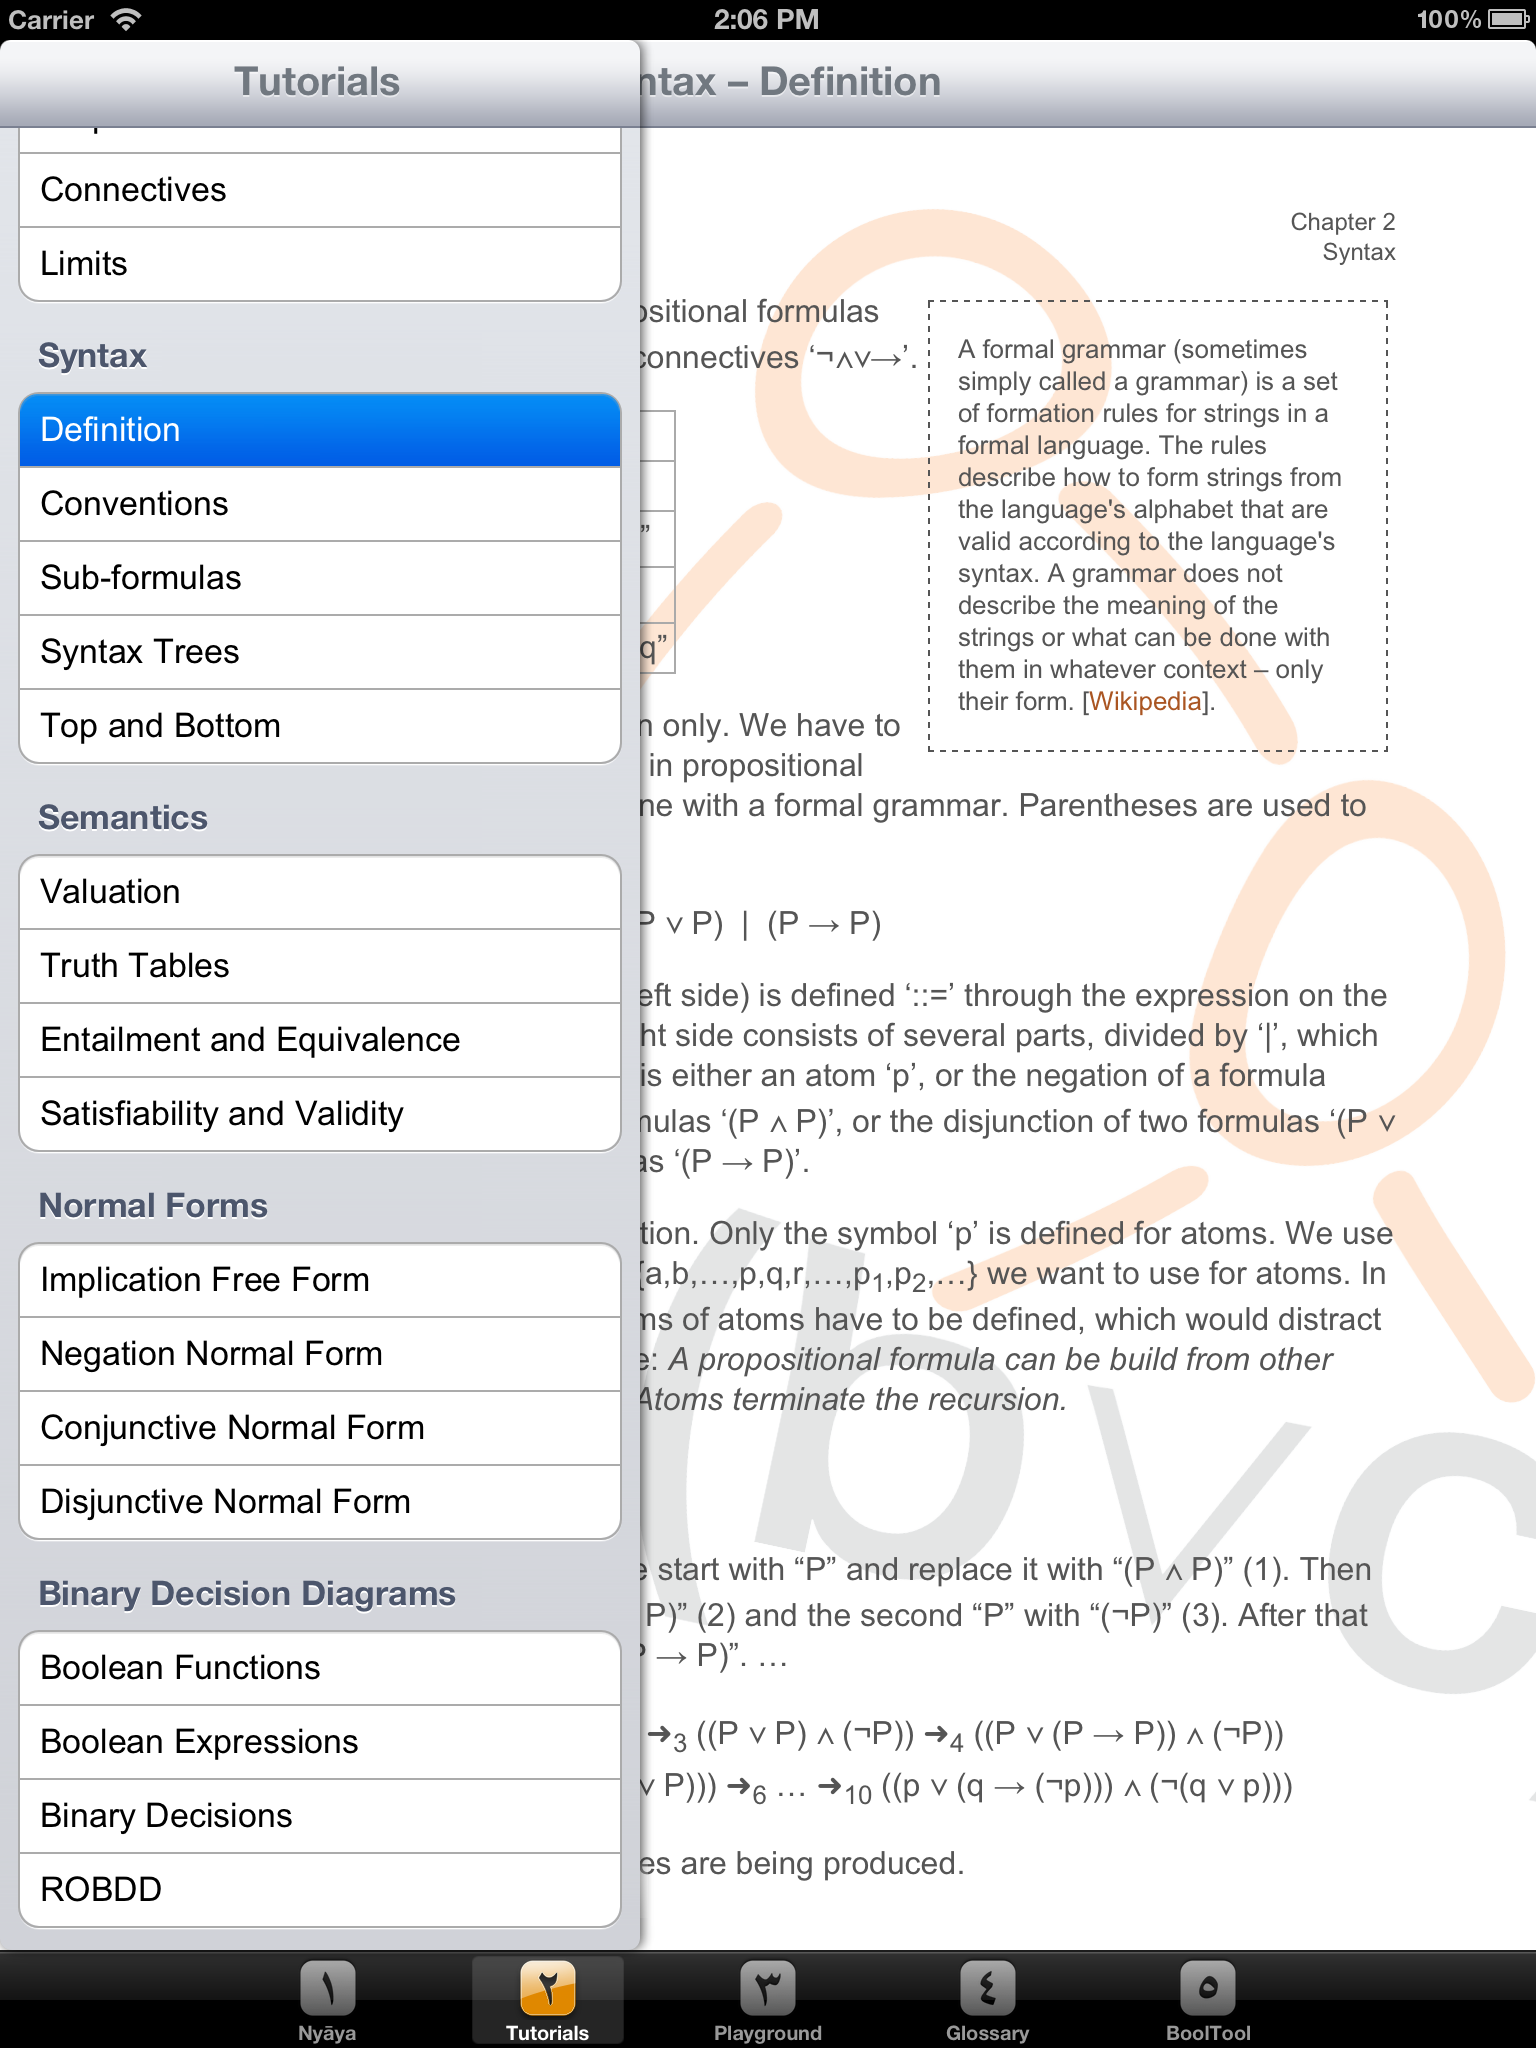
\includegraphics[width=12cm]{pics/S_Tutorials.png}
\caption{Tutorial}
\label{fig:ScreenshotTutorials}
\end{center}
\end{figure}

\begin{figure}[htbp]
\begin{center}
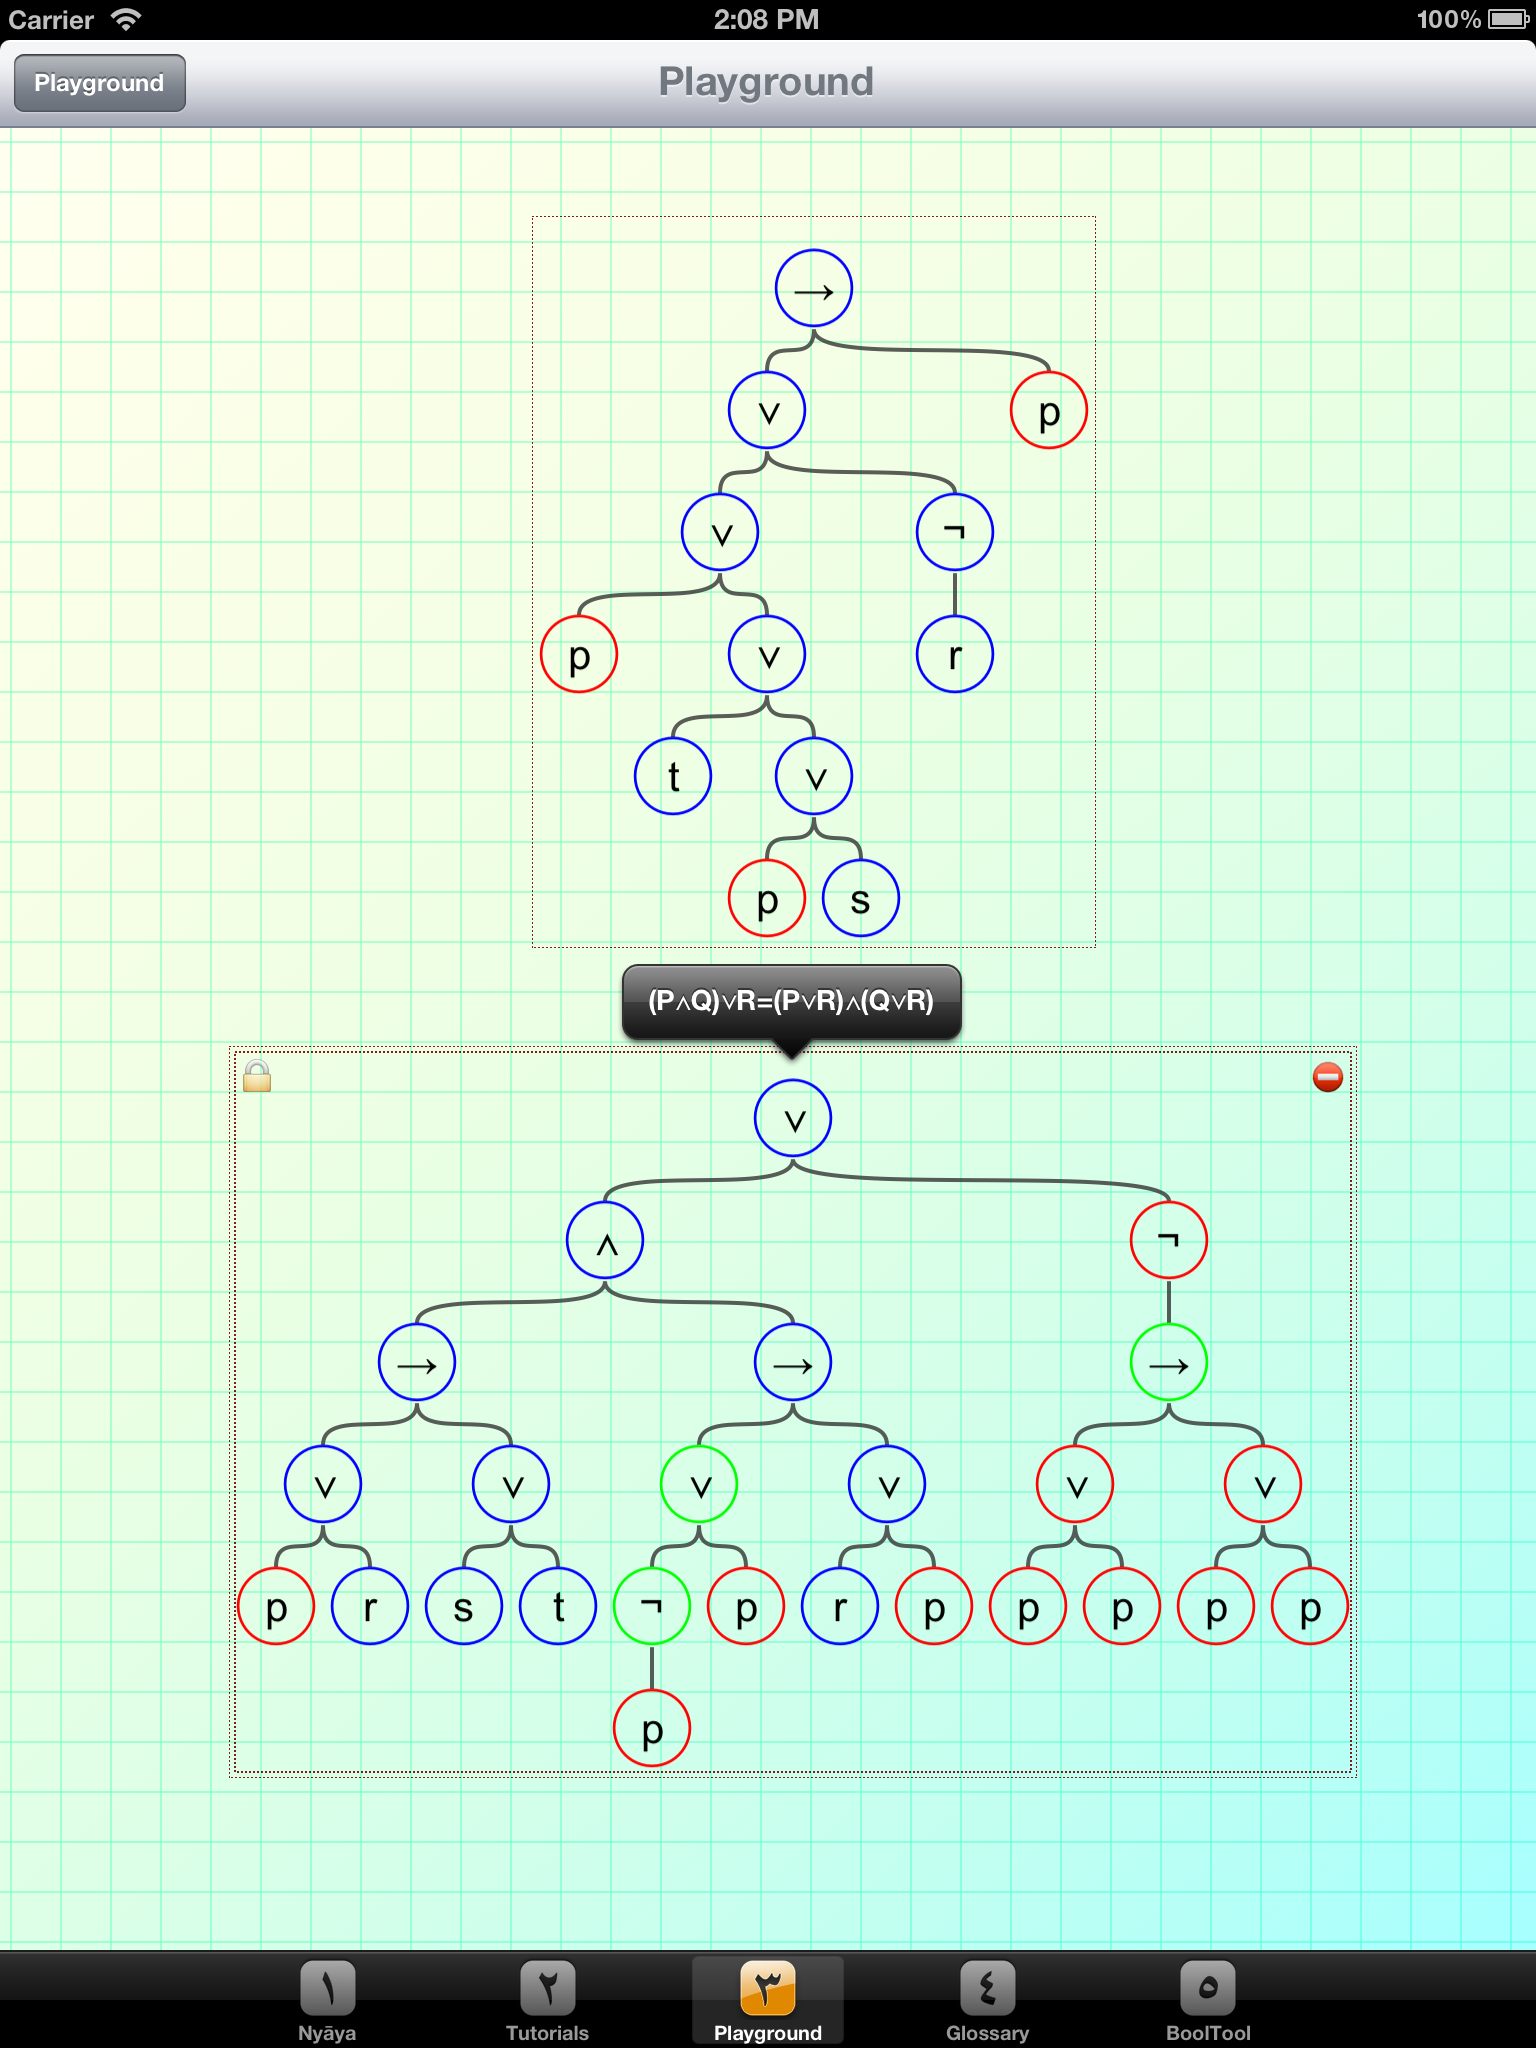
\includegraphics[width=12cm]{pics/S_Playground.png}
\caption{Playground}
\label{fig:ScreenshotPlayground}
\end{center}
\end{figure}

\begin{figure}[htbp]
\begin{center}
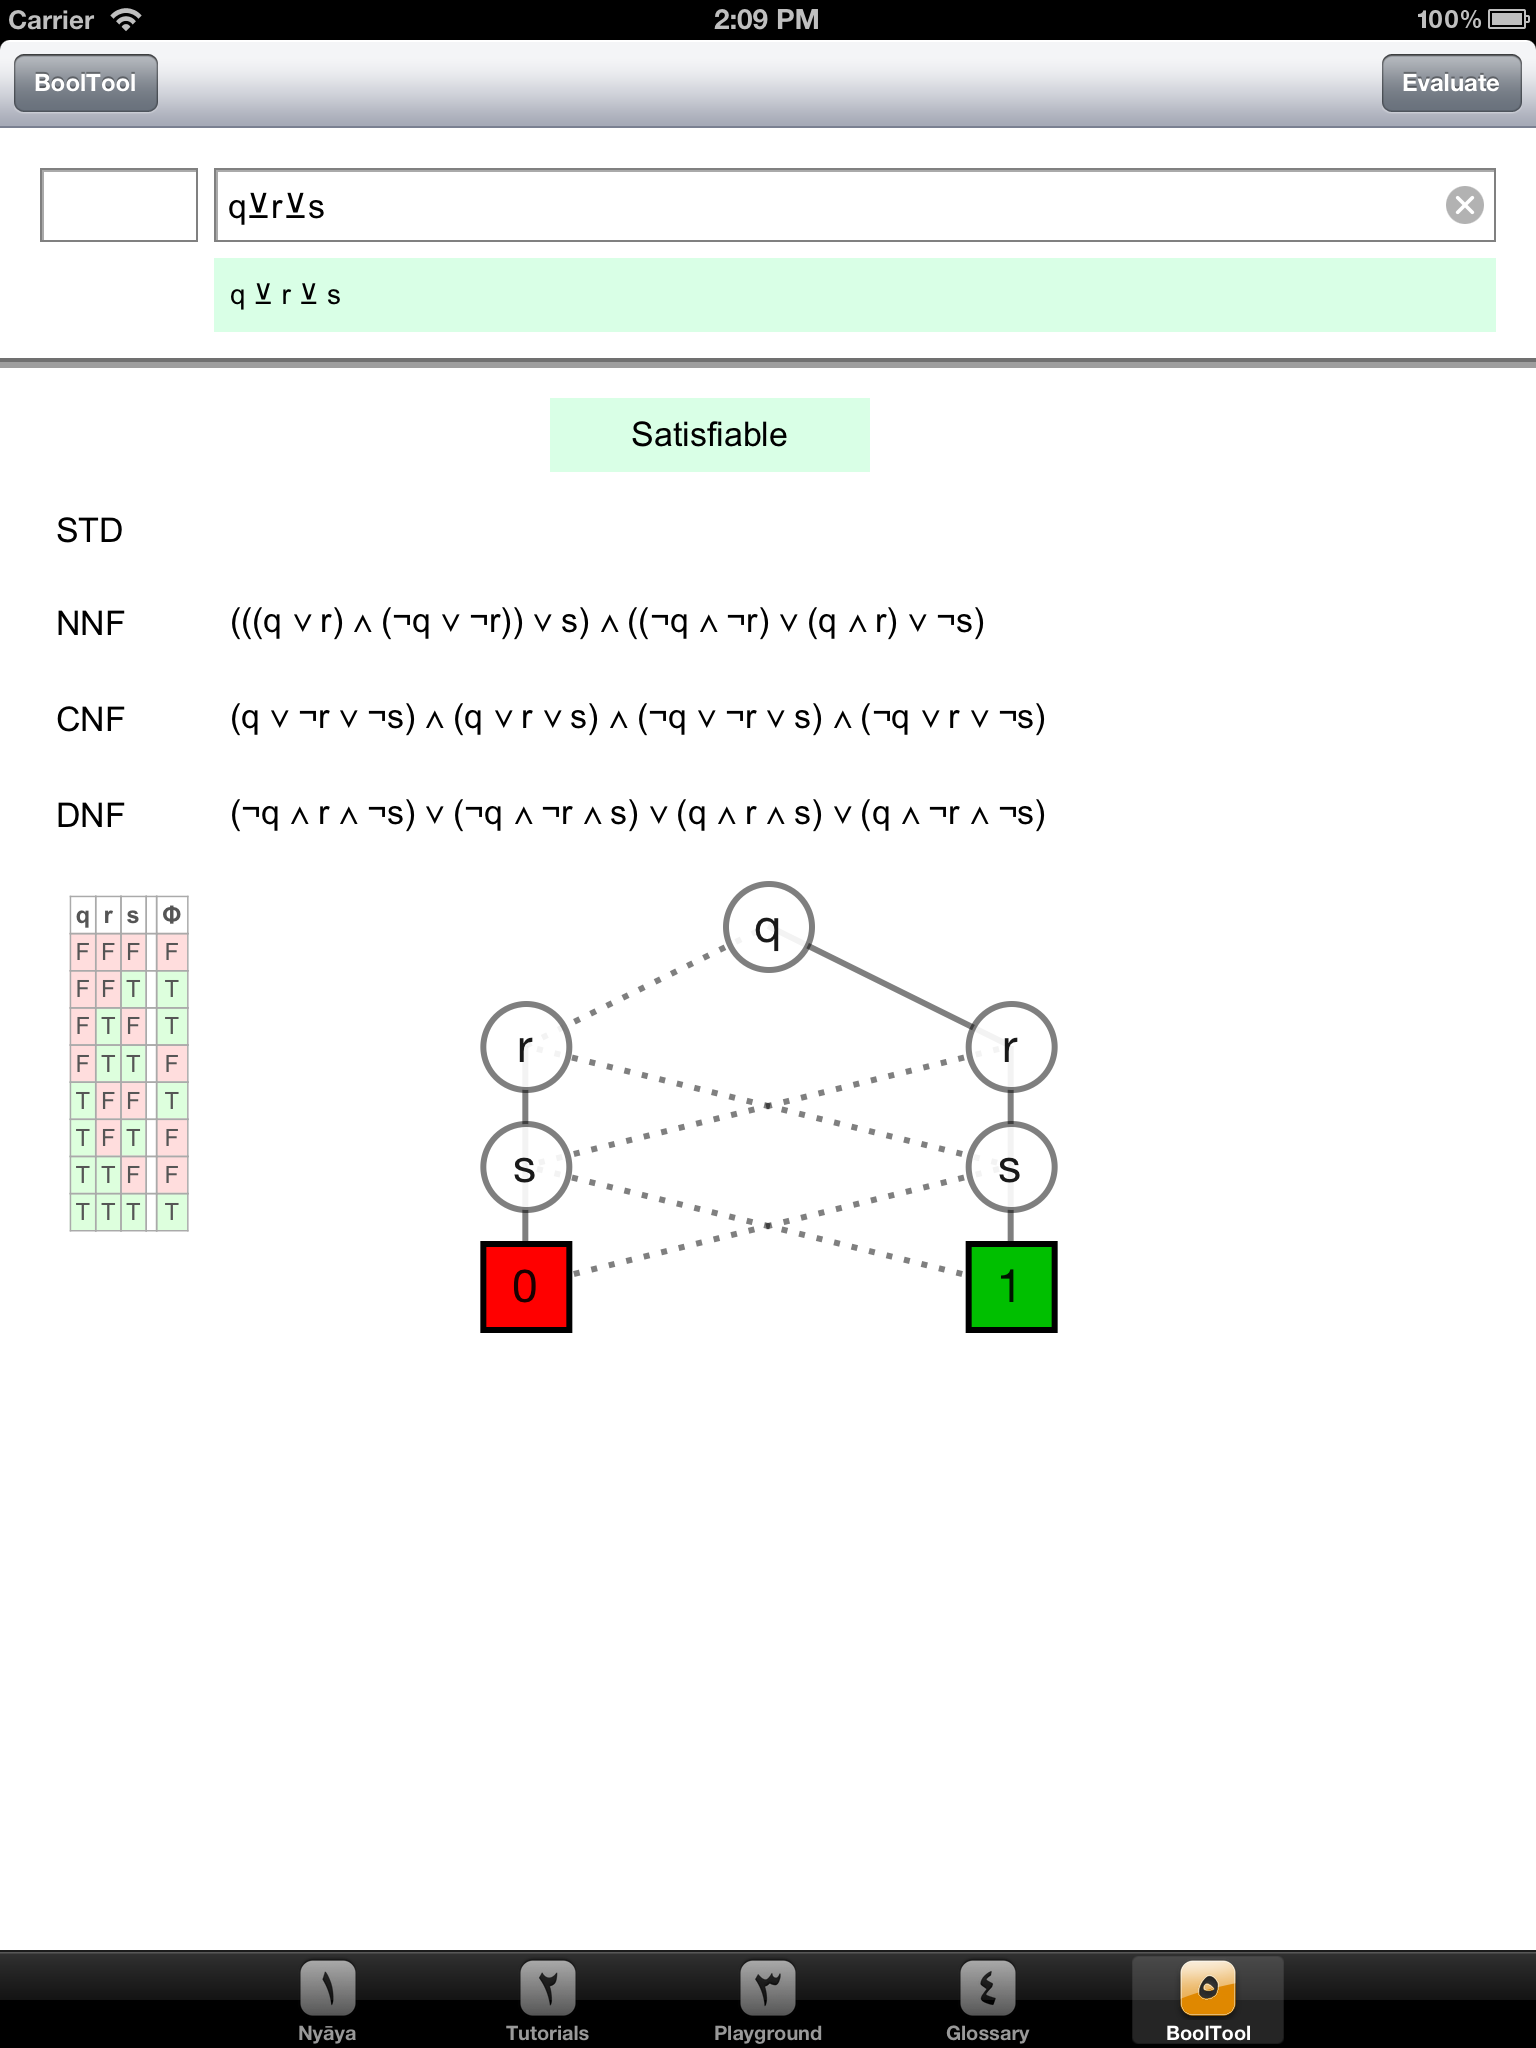
\includegraphics[width=12cm]{pics/S_BoolTool.png}
\caption{BoolTool}
\label{fig:ScrrenshotBoolTool}
\end{center}
\end{figure}



